\documentclass{standalone}
\usepackage{tikz}
\usepackage{fontspec}

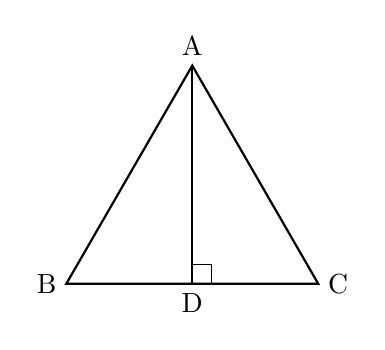
\begin{tikzpicture}[scale=0.8]
    % সমবাহু ত্রিভুজ ABC অঙ্কন
    \coordinate (B) at (0,0);
    \coordinate (C) at (4,0);
    \coordinate (A) at (2, 3.464);
    \coordinate (D) at (2,0);
    
    \draw[thick] (A) -- (B) -- (C) -- cycle;
    \draw[thick] (A) -- (D); % উচ্চতা AD
    
    % লেবেলসমূহ
    \node[above] at (A) {A};
    \node[left] at (B) {B};
    \node[right] at (C) {C};
    \node[below] at (D) {D};
    
    % সমকোণ চিহ্ন
    \draw (2, 0.3) -- (2.3, 0.3) -- (2.3, 0);
    
\end{tikzpicture}
\end{document}
